\documentclass{ximera}
%\auor{Matthew Charnley and Jason Nowell}
\usepackage[margin=1.5cm]{geometry}
\usepackage{indentfirst}
\usepackage{sagetex}
\usepackage{lipsum}
\usepackage{amsmath}
\usepackage{mathrsfs}


%%% Random packages added without verifying what they are really doing - just to get initial compile to work.
\usepackage{tcolorbox}
\usepackage{hypcap}
\usepackage{booktabs}%% To get \toprule,\midrule,\bottomrule etc.
\usepackage{nicefrac}
\usepackage{caption}
\usepackage{units}

% This is my modified wrapfig that doesn't use intextsep
\usepackage{mywrapfig}
\usepackage{import}



%%% End to random added packages.


\graphicspath{
    {./figures/}
    {./../figures/}
    {./../../figures/}
}
\renewcommand{\log}{\ln}%%%%
\DeclareMathOperator{\arcsec}{arcsec}
%% New commands


%%%%%%%%%%%%%%%%%%%%
% New Conditionals %
%%%%%%%%%%%%%%%%%%%%


% referencing
\makeatletter
    \DeclareRobustCommand{\myvref}[2]{%
      \leavevmode%
      \begingroup
        \let\T@pageref\@pagerefstar
        \hyperref[{#2}]{%
	  #1~\ref*{#2}%
        }%
        \vpageref[\unskip]{#2}%
      \endgroup
    }%

    \DeclareRobustCommand{\myref}[2]{%
      \leavevmode%
      \begingroup
        \let\T@pageref\@pagerefstar
        \hyperref[{#2}]{%
	  #1~\ref*{#2}%
        }%
      \endgroup
    }%
\makeatother

\newcommand{\figurevref}[1]{\myvref{Figure}{#1}}
\newcommand{\figureref}[1]{\myref{Figure}{#1}}
\newcommand{\tablevref}[1]{\myvref{Table}{#1}}
\newcommand{\tableref}[1]{\myref{Table}{#1}}
\newcommand{\chapterref}[1]{\myref{chapter}{#1}}
\newcommand{\Chapterref}[1]{\myref{Chapter}{#1}}
\newcommand{\appendixref}[1]{\myref{appendix}{#1}}
\newcommand{\Appendixref}[1]{\myref{Appendix}{#1}}
\newcommand{\sectionref}[1]{\myref{\S}{#1}}
\newcommand{\subsectionref}[1]{\myref{subsection}{#1}}
\newcommand{\subsectionvref}[1]{\myvref{subsection}{#1}}
\newcommand{\exercisevref}[1]{\myvref{Exercise}{#1}}
\newcommand{\exerciseref}[1]{\myref{Exercise}{#1}}
\newcommand{\examplevref}[1]{\myvref{Example}{#1}}
\newcommand{\exampleref}[1]{\myref{Example}{#1}}
\newcommand{\thmvref}[1]{\myvref{Theorem}{#1}}
\newcommand{\thmref}[1]{\myref{Theorem}{#1}}


\renewcommand{\exampleref}[1]{ {\color{red} \bfseries Normally a reference to a previous example goes here.}}
\renewcommand{\figurevref}[1]{ {\color{red} \bfseries Normally a reference to a previous figure goes here.}}
\renewcommand{\tablevref}[1]{ {\color{red} \bfseries Normally a reference to a previous table goes here.}}
\renewcommand{\Appendixref}[1]{ {\color{red} \bfseries Normally a reference to an Appendix goes here.}}
\renewcommand{\exercisevref}[1]{ {\color{red} \bfseries Normally a reference to a previous exercise goes here.}}



\newcommand{\R}{\mathbb{R}}

%% Example Solution Env.
\def\beginSolclaim{\par\addvspace{\medskipamount}\noindent\hbox{\bf Solution:}\hspace{0.5em}\ignorespaces}
\def\endSolclaim{\par\addvspace{-1em}\hfill\rule{1em}{0.4pt}\hspace{-0.4pt}\rule{0.4pt}{1em}\par\addvspace{\medskipamount}}
\newenvironment{exampleSol}[1][]{\beginSolclaim}{\endSolclaim}

%% General figure formating from original book.
\newcommand{\mybeginframe}{%
\begin{tcolorbox}[colback=white,colframe=lightgray,left=5pt,right=5pt]%
}
\newcommand{\myendframe}{%
\end{tcolorbox}%
}

%%% Eventually return and fix this to make matlab code work correctly.
%% Define the matlab environment as another code environment
%\newenvironment{matlab}
%{% Begin Environment Code
%{ \centering \bfseries Matlab Code }
%\begin{code}
%}% End of Begin Environment Code
%{% Start of End Environment Code
%\end{code}
%}% End of End Environment Code


% this one should have a caption, first argument is the size
\newenvironment{mywrapfig}[2][]{
 \wrapfigure[#1]{r}{#2}
 \mybeginframe
 \centering
}{%
 \myendframe
 \endwrapfigure
}

% this one has no caption, first argument is size,
% the second argument is a larger size used for HTML (ignored by latex)
\newenvironment{mywrapfigsimp}[3][]{%
 \wrapfigure[#1]{r}{#2}%
 \centering%
}{%
 \endwrapfigure%
}
\newenvironment{myfig}
    {%
    \begin{figure}[h!t]
        \mybeginframe%
        \centering%
    }
    {%
        \myendframe
    \end{figure}%
    }


% graphics include
\newcommand{\diffyincludegraphics}[3]{\includegraphics[#1]{#3}}
\newcommand{\myincludegraphics}[3]{\includegraphics[#1]{#3}}
\newcommand{\inputpdft}[1]{\subimport*{../figures/}{#1.pdf_t}}


%% Not sure what these even do? They don't seem to actually work... fun!
%\newcommand{\mybxbg}[1]{\tcboxmath[colback=white,colframe=black,boxrule=0.5pt,top=1.5pt,bottom=1.5pt]{#1}}
%\newcommand{\mybxsm}[1]{\tcboxmath[colback=white,colframe=black,boxrule=0.5pt,left=0pt,right=0pt,top=0pt,bottom=0pt]{#1}}
\newcommand{\mybxsm}[1]{#1}
\newcommand{\mybxbg}[1]{#1}

%%% Something about tasks for practice/hw?
\usepackage{tasks}
\usepackage{footnote}
\makesavenoteenv{tasks}


%% For pdf only?
\newcommand{\diffypdfversion}[1]{#1}


%% Kill ``cite'' and go back later to fix it.
\renewcommand{\cite}[1]{}


%% Currently we can't really use index or its derivatives. So we are gonna kill them off.
\renewcommand{\index}[1]{}
\newcommand{\myindex}[1]{#1}






\title{Polynomials and Factoring}
\author{Matthew Charnley and Jason Nowell}


%\outcome{Use power series methods to solve second order linear ODEs near ordinary points}
%\outcome{Write a recurrence relation for the coefficients in a power series solution to an ODE.}


\begin{document}
\begin{abstract}
    We review Polynomials and Factoring
\end{abstract}
\maketitle

\label{sec:polys}

%\sectionnotes{Attribution: \cite{SZ}, \S A.8, A.9, 2.2-2.4}

There are several components of differential equations, particularly higher order equations and systems, that involve dealing with and finding roots of polynomials, using these results to generate solutions to differential equations. This appendix will review some properties of and techniques related to polynomials. 

\subsection{Definitions and Operations}

First we start with the definition of a polynomial. A \emph{polynomial}\index{polynomial} is a sum of terms each of which is a real number or a real number multiplied by one or more variables to natural number powers. Some examples of polynomials are $x^2 + x\sqrt{3} + 4$, $27x^2y + \frac{7x}{2}$ and $6$. Things like $3\sqrt{x}$, $4x - \frac{2}{x+1}$ and $13x^{2/3}y^{2}$ are \emph{not} polynomials. Below, we review some terminology about polynomials.
\begin{definition}
    \begin{itemize}
        \item  Terms in polynomials without variables are called \emph{constant}\index{polynomial ! constant} terms.
        \item  In non-constant terms, the real number factor in the expression is called the \emph{coefficient}\index{polynomial ! coefficient} of the term. 
        \item  The \emph{degree}\index{polynomial ! degree} of a non-constant term is the sum of the exponents on the variables in the term; non-zero constant terms are defined to have degree $0$. The degree of a polynomial is the highest degree of the nonzero terms.
        \item  Terms in a polynomial are called \emph{like}\index{term ! like} terms if they have the same variables each with the same corresponding exponents.
        \item  A polynomial is said to be \emph{simplified}\index{polynomial ! simplified} if all arithmetic operations have been completed and there are no longer any like terms.
        \item  A simplified polynomial  is  called a 
        \begin{itemize}
            \item   \emph{monomial}\index{monomial} if it has exactly one nonzero term
            \item   \emph{binomial}\index{binomial} if it has exactly two nonzero terms
            \item   \emph{trinomial}\index{trinomial} if it has exactly three nonzero terms
        \end{itemize}
    \end{itemize}
\end{definition}

For example, $x^2 + x\sqrt{3} +4$ is a trinomial of degree $2$.  The coefficient of $x^2$ is $1$ and the constant term is $4$.  The polynomial $27x^2y + \frac{7x}{2}$ is a binomial of degree $3$ ($x^2y = x^2 y^1$) with constant term $0$.  

The concept of `like' terms really amounts to finding terms which can be combined using the Distributive Property.  For example, in the polynomial $17x^2y - 3xy^2 + 7xy^2$, $-3xy^2$ and $7xy^2$ are like terms, since they have the same variables with the same corresponding exponents. This allows us to combine these two terms as follows:  
\[
    17x^2y -  3xy^2 + 7xy^2 = 17x^2y + (-3)xy^2 + 7xy^2 + 17x^2y +(-3 + 7)xy^2 = 17x^2y + 4xy^2
\]  
Note that even though $17x^2y$ and $4xy^2$ have the same variables, they are not like terms since in the first term we have $x^2$ and $y = y^1$ but in the second we have $x = x^1$ and $y = y^2$ so the corresponding exponents aren't the same.  Hence,  $17x^2y + 4xy^2$ is the simplified form of the polynomial.  

There are four basic operations we can perform with polynomials:  addition, subtraction, multiplication and division. Addition, subtraction, and multiplication follow the standard properties of real numbers after distributing or expanding all terms (for multiplication) and then collecting like terms again. Division, on the other hand, is a bit more complicated and will be discussed next.

\subsubsection{Polynomial Long Division}

We now turn our attention to polynomial long division.  Dividing two polynomials follows the same algorithm, in principle, as dividing two natural numbers so we review that process first.  Suppose we wished to divide $2585$ by $79$.  The standard division tableau is given below. 
\setlength\arraycolsep{0.1pt}
\setlength\extrarowheight{2pt}
\[ 
    \begin{array}{cccccc}
        &             &     &   & 3 & 2  \\ \hhline{~~|----}
      7 & 9  \vline & 2 & 5 & 8 & 5  \\
        &            -&   2 & 3 & 7 & \downarrow \\ \hhline{~~---} 
        &             &     & 2 & 1 &  5   \\ 
        &             &   - & 1 & 5 & 8    \\ \hhline{~~~---} 
        &             &     &   & 5 & 7    \\
    \end{array}
\]

\setlength\arraycolsep{5pt}
\setlength\extrarowheight{0pt}

In this case, $79$ is called the \emph{divisor}\index{division ! divisor}, $2585$ is called the \emph{dividend}\index{division ! dividend}, $32$ is called the \emph{quotient}\index{division ! quotient} and $57$ is called the \emph{remainder}\index{division ! remainder}.  We can check our answer by showing:  
\[ 
    \text{dividend} = (\text{divisor})( \text{quotient}) + \text{remainder}
\] 
or in this case, $2585 = (79)(32) + 57 \checkmark$.  We hope that the long division tableau evokes warm, fuzzy memories of your formative years as opposed to feelings of hopelessness and frustration.  If you experience the latter, keep in mind that the Division Algorithm essentially is a two-step process, iterated over and over again.  First, we guess the number of times the divisor goes into the dividend and  then we subtract off our guess.  We repeat those steps with what's left over until what's left over (the remainder) is less than what we started with (the divisor).  That's all there is to it!

The division algorithm for polynomials has the same basic two steps but when we subtract polynomials, we must take care to subtract \emph{like terms} only.  As a transition to polynomial division, let's write out our previous division tableau in expanded form.


\setlength\arraycolsep{0.1pt}
\setlength\extrarowheight{2pt}

\[ 
\begin{array}{cccccccccc}
            & &         &                           & &                           & & 3 \cdot 10                &+& 2 \\ \hhline{~~~|-------}
7 \cdot 10  &+& 9\vline & 2\cdot 10^3               &+& 5 \cdot 10^2              &+& 8 \cdot 10                &+& 5 \\
            & & -       & \left(2 \cdot 10^3 \right.&+&  3 \cdot 10^2             &+& \left. 7 \cdot 10 \right) & &  \downarrow \\ \hhline{~~~-----~~} 
            & &         &                           & & 2 \cdot 10^2              &+& 1 \cdot 10                &+& 5 \\ 
            & &         &                           &-& \left(1 \cdot 10^2 \right.&+&  5 \cdot 10               &+&\left.  8 \right) \\ \hhline{~~~~~---~~} 
            & &         &                           & &  & & 5 \cdot 10           &+& 7 \\
\end{array}
\]

\setlength\arraycolsep{5pt}
\setlength\extrarowheight{0pt}

Written this way, we see that when we line up the digits we are really lining up the coefficients of the corresponding powers of $10$ - much like how we'll have to keep the powers of $x$ lined up in the same columns.  The big difference between polynomial division and the division of natural numbers is that the value of $x$ is an unknown quantity.  So unlike using the known value of $10$, when we subtract there can be no regrouping of coefficients as in our previous example. (The subtraction $215 - 158$ requires us to `regroup' or `borrow' from the tens digit, then the hundreds digit.) This actually makes polynomial division easier.%
\footnote{In our opinion - you can judge for yourself.}
Before we dive into examples, we first state a theorem telling us when we can divide two polynomials, and what to expect when we do so.

\begin{theorem}[Polynomial Division]
    \label{polydiv}
    Let $d$ and $p$ be nonzero polynomials where the degree of $p$ is greater than or equal to the degree of $d$.  There exist two unique polynomials, $q$ and $r$, such that $p = d \cdot q + r,$ where either $r = 0$ or the degree of $r$ is strictly less than the degree of $d$.
\end{theorem}

Essentially, Theorem \ref{polydiv} tells us that we can divide polynomials whenever the degree of the divisor is less than or equal to the degree of the dividend.  We know we're done with the division when the polynomial left over (the remainder) has a degree strictly less than the divisor.  It's time to walk through a few examples to refresh your memory.

\begin{example}
    \label{polynomiallongdivex}  Perform the indicated division.  Check your answer by showing 
    \[
        \text{dividend} = (\text{divisor})( \text{quotient}) + \text{remainder}
    \]
    \newcounter{HW}
    \begin{multicols}{2}
        \begin{enumerate}
            \item  $\left(x^3 + 4x^2 - 5x - 14\right) \div (x-2)$
            \item  $\left(2t +  7\right) \div \left(3t - 4\right)$
        \end{enumerate}
    \end{multicols}
    \begin{multicols}{2}
        \begin{enumerate}
            \item  $\left(6y^2 - 1 \right) \div \left(2y + 5\right)$
            \item  $\left(w^3 \right) \div \left(w^2 - \sqrt{2}\right)$.
        \end{enumerate}
    \end{multicols}
\end{example}

\begin{exampleSol}
    \begin{enumerate}
        \item  To begin $\left(x^3 + 4x^2 - 5x - 14\right) \div (x-2)$, we divide the first term in the dividend, namely $x^3$, by the first term in the divisor, namely $x$, and get $\frac{x^3}{x} = x^2$. This then becomes the first term in the quotient.  We proceed as in regular long division at this point: we multiply the entire divisor, $x-2$, by this first term in the quotient to get $x^{2}(x - 2) = x^3 - 2x^2$.  We then subtract this result from the dividend.
            
            \setlength\arraycolsep{0.1pt}\setlength\extrarowheight{2pt}
            \[ 
            \begin{array}{cccccccccc}
            & & & & & x^2 & & &  &  \\ \hhline{~~~|-------}
            x & - & 2  \vline& x^3 & + & 4x^2 & - & 5x & - & 14 \\
             &  &  -& \left(x^3 \right. & - & \left.  2x^2\right) &  & \downarrow &  &  \\ \hhline{~~~---~~~~} 
             &  &  &   &  & 6 x^2 & - & 5x &  &  \\ 
            % &  &  &   & - & \left(6 x^2 \right. & - & \left. 12x \right) &  &  \\ \hhline{~~~~~---~~} 
            % &  &  &   &   &  & & 7x  & - & 14 \\
            % &  &  &   &   &  & - & \left( 7x \right. & - & \left. 14 \right) \\ \hhline{~~~~~~~---} 
            % &   &  &  &  &  &  &  &  & 0
            \end{array}
            \]
            
            \setlength\arraycolsep{5pt}
            \setlength\extrarowheight{0pt} 
            
            Now we `bring down' the next term of the quotient, namely $-5x$, and repeat the process. We divide $\frac{6x^2}{x} = 6x$, and add this to the quotient polynomial, multiply it by the divisor (which yields $6x(x - 2) = 6x^{2} - 12x$) and subtract. \setlength\arraycolsep{0.1pt}\setlength\extrarowheight{2pt}
            
            \[ 
            \begin{array}{cccccccccc}
                & & & & & x^2 & + & 6x &  &  \\ \hhline{~~~|-------}
                x & - & 2  \vline& x^3 & + & 4x^2 & - & 5x & - & 14 \\
                &  &  -& \left(x^3 \right. & - & \left.  2x^2\right) &  & &  & \downarrow  \\ \hhline{~~~---~~~~} 
                &  &  &   &  & 6 x^2 & - & 5x &  &  \downarrow \\ 
                &  &  &   & - & \left(6 x^2 \right. & - & \left. 12x \right) &  & \downarrow \\ \hhline{~~~~~---~~} 
                &  &  &   &   &  & & 7x  & - & 14 \\
                % &  &  &   &   &  & - & \left( 7x \right. & - & \left. 14 \right) \\ \hhline{~~~~~~~---} 
                % &   &  &  &  &  &  &  &  & 0 
            \end{array}
            \]
            
            \setlength\arraycolsep{5pt}
            \setlength\extrarowheight{0pt}
            
            Finally, we `bring down' the last term of the dividend, namely $-14$, and repeat the process.  We divide $\frac{7x}{x} = 7$, add this to the quotient, multiply it by the divisor (which yields $7(x - 2) = 7x - 14$) and subtract.\setlength\arraycolsep{0.1pt}\setlength\extrarowheight{2pt}
            
            \[ 
            \begin{array}{cccccccccc}
                & & & & & x^2 & + & 6x & + & 7 \\ \hhline{~~~|-------}
                x & - & 2  \vline& x^3 & + & 4x^2 & - & 5x & - & 14 \\
                &  &  -& \left(x^3 \right. & - & \left.  2x^2\right) &  &  &  &  \\ \hhline{~~~---~~~~} 
                &  &  &   &  & 6 x^2 & - & 5x &  &  \\ 
                &  &  &   & - & \left(6 x^2 \right. & - & \left. 12x \right) &  &  \\ \hhline{~~~~~---~~} 
                &  &  &   &   &  & & 7x  & - & 14 \\
                &  &  &   &   &  & - & \left( 7x \right. & - & \left. 14 \right) \\ \hhline{~~~~~~~---} 
                &   &  &  &  &  &  &  &  & 0
            \end{array}
            \]
            \setlength\arraycolsep{5pt}
            \setlength\extrarowheight{0pt}
            
            In this case, we get a quotient of $x^2 + 6x + 7$ with a remainder of $0$.  To check our answer, we compute  \[(x-2)\left(x^2 + 6x + 7\right) + 0 = x^3 + 6x^2 + 7x - 2x^2 - 12x -14 =  x^3 + 4x^2 - 5x - 14  \checkmark \]
            
        \item To compute  $\left(2t +  7\right) \div \left(3t - 4\right)$, we start as before.  We find $\frac{2t}{3t} = \frac{2}{3}$, so that becomes the first (and only) term in the quotient.  We multiply the divisor $(3t-4)$ by $\frac{2}{3}$ and get $2t - \frac{8}{3}$.  We subtract this from the divided and get $\frac{29}{3}$.
            
            \setlength\arraycolsep{0.1pt}\setlength\extrarowheight{5pt}
            
            \[ 
            \begin{array}{cccccc}
                & & & & & \dfrac{2}{3} \\ \hhline{~~~|---}
                3t & - & 4  \vline& 2t & + & 7  \\
                &  &  -& \left(2t\vphantom{\dfrac{8}{3}} \right. & - & \left.  \dfrac{8}{3}\right)  \\ \hhline{~~~---}
                &  &  &   &  & \dfrac{29}{3} \vphantom{\sqrt{\dfrac{7}{7}}} \\ 
            \end{array}
            \]
            \setlength\arraycolsep{5pt}
            \setlength\extrarowheight{0pt}
            
            Our answer is $\frac{2}{3}$ with a remainder of $\frac{29}{3}$.  To check our answer, we compute 
            \[
                (3t-4) \left(\frac{2}{3}\right) + \frac{29}{3} = 2t - \frac{8}{3} + \frac{29}{3} = 2t + \frac{21}{3} = 2t + 7  \checkmark
            \]
        
        \item When we set-up the tableau for   $\left(6y^2 - 1 \right) \div \left(2y + 5\right)$, we must first issue a `placeholder' for the `missing' $y$-term in the dividend, $6y^2 -1 = 6y^2 + 0y - 1$.  We then proceed as before.  Since $\frac{6y^2}{2y} = 3y$, $3y$ is the first term in our quotient. We multiply $(2y+5)$ times $3y$ and subtract it from the dividend.  We bring down the $-1$, and repeat.  
        
            \setlength\arraycolsep{0.1pt}\setlength\extrarowheight{5pt}
            \[ 
            \begin{array}{cccccccc}
                & & & & & 3y & - & \dfrac{15}{2}  \\ \hhline{~~~|-----}
                2y& + & 5  \vline& 6y^2 & + & 0y & - & 1  \\
                &  &  -& \left(6y^2 \right. & + & \left.  15y\right) &  & \downarrow  \\ \hhline{~~~---~~} 
                &  &  &   &  & -15y & - & 1  \\ 
                &  &  &   & - & \left(-15y\vphantom{\dfrac{75}{2}} \right. & - & \left. \dfrac{75}{2} \right) \\ \hhline{~~~~~---} 
                &  &  &   &   &  & & \dfrac{73}{2} \vphantom{\sqrt{\dfrac{73}{2}}}\\
            \end{array}
            \]
            \setlength\arraycolsep{5pt}
            \setlength\extrarowheight{0pt}
             
            Our answer is $3y - \frac{15}{2}$ with a remainder of $\frac{73}{2}$.  To check our answer, we compute:
            
            \[ 
                (2y + 5)\left(3y - \dfrac{15}{2}\right) + \dfrac{73}{2} = 6y^2 - 15y + 15y - \dfrac{75}{2} + \dfrac{73}{2} = 6y^2 - 1  \checkmark
            \]
            
        \item For our last example, we need `placeholders' for both the divisor  $w^2 - \sqrt{2} = w^2 + 0w -\sqrt{2}$ and the dividend $w^3 = w^3 + 0w^2 + 0w + 0$.  The first term in the quotient is $\frac{w^3}{w^2} = w$, and when we multiply and subtract this from the dividend, we're left with just $0w^2 + w\sqrt{2} + 0 = w\sqrt{2}$.
            
            \setlength\arraycolsep{0.1pt}
            \setlength\extrarowheight{2pt}
            
            \[ 
            \begin{array}{cccccccccccc}
                &   &    &   &                    &     &   &      &   &  w &   & \\ \hhline{~~~~~|-------}
                w^2 & + & 0w & - & \sqrt{2}  \vline & w^3 & + & 0w^2 & + & 0w & + & 0  \\
                &   &    &    &                  -&\left(w^3\vphantom{w\sqrt{2}} \right. & + & 0w^2 & - & \left.  w\sqrt{2} \right) & & \downarrow \\ \hhline{~~~~~-----~~}
                &   &    &    &                   &                                       &  &  0w^2     &  + &   w\sqrt{2}  & + & 0\\ 
            \end{array}
            \]
            \setlength\arraycolsep{5pt}
            \setlength\extrarowheight{0pt}
            
            Since the degree of $w\sqrt{2}$ (which is $1$) is less than the degree of the divisor (which is $2$), we are done.\footnote{Since $\frac{0w^2}{w^2} = 0$, we could proceed, write our quotient as $w+0$, and move on\ldots but even pedants have limits.}  Our answer is $w$ with a remainder of $w \sqrt{2}$.  To check, we compute:
            
            \[ 
                \left(w^2 - \sqrt{2}\right)w + w\sqrt{2} = w^3 - w\sqrt{2} + w\sqrt{2} = w^3  \checkmark
            \]
    \end{enumerate}
\end{exampleSol}


\subsection{Synthetic Division}

Usually, when we want to divide polynomials, it is because we are trying to find all roots of a polynomial. This comes from the idea that if we have a polynomial $p(x)$ and a value $x_0$ so that $p(x_0) = 0$, then $x_0$ is a root of the polynomial. This means that $(x-x_0)$ is a factor of $p(x)$, so that we can write 
\[ 
    p(x) = (x-x_0)q(x) 
\] 
where $q(x)$ is a polynomial with one lower degree than $p$. We can find this $q(x)$ by dividing
\[ 
    q(x) = \frac{p(x)}{x-x_0}, 
\] 
which is why we need division to sort this out. 

This means that we need to find the roots (or at least a root) to know what to divide $p(x)$ by in order to start this process. The main theorem that can tell us where to start is the Rational Roots Theorem. 

\begin{theorem}[Rational Zeros Theorem]
    \label{RZT}
    \index{Rational Zeros Theorem} Suppose $f(x) = a_{n} x^{n} + a_{n-\mbox{\tiny$1$}}x^{n-\mbox{\tiny$1$}} + \ldots + a_{\mbox{\tiny$1$}} x + a_{\mbox{\tiny$0$}}$ is a polynomial of degree $n$ with $n \geq 1$, and $a_{\mbox{\tiny$0$}}$, $a_{\mbox{\tiny$1$}}$, \ldots $a_{n}$ are integers.  If $r$ is a rational zero of $f$, then $r$ is of the form $\pm \frac{p}{q}$, where $p$ is a factor of the constant term $a_{\mbox{\tiny$0$}}$, and $q$ is a factor of the leading coefficient $a_{n}$.  
\end{theorem}

The Rational Zeros Theorem gives us a list of numbers to try in our synthetic division and that is a lot nicer than simply guessing.  If none of the numbers in the list are zeros, then either the polynomial has no real zeros at all, or all of the real zeros are irrational numbers.

\begin{example}
    Let $f(x) = 2x^4+4x^3-x^2-6x-3$. Use the Rational Zeros Theorem to list all of the possible rational zeros of $f$.
\end{example}

\begin{exampleSol}
    To generate a complete list of rational zeros, we need to take each of the factors of constant term, $a_{\mbox{\tiny$0$}} = -3$, and divide them by each of the factors of the leading coefficient $a_{\mbox{\tiny$4$}} = 2$.  The factors of $-3$ are $\pm  1$ and $\pm  3$.  Since the Rational Zeros Theorem tacks on a $\pm$ anyway, for the moment, we consider only the positive factors $1$ and $3$.  The factors of $2$ are  $1$ and $2$, so the Rational Zeros Theorem gives the list 
    $\left\{\pm  \frac{1}{1}, \pm  \frac{1}{2},  \pm  \frac{3}{1}, \pm  \frac{3}{2}\right\}$ or $\left\{\pm  \frac{1}{2}, \pm  1, \pm  \frac{3}{2}, \pm  3\right\}$.   
    \label{RZTex}
\end{exampleSol}

But this still doesn't make the process easy or straight-forward for finding the roots. How can we take this list of options and easily figure out where the roots are, and what the remaining polynomial $q(x)$ is?

We start by way of example:  suppose we wish to determine the zeros of  $f(x) = x^3 + 4x^2-5x-14$.  Setting $f(x)=0$ results in the polynomial equation $x^3 + 4x^2-5x-14=0$.   Despite all of the factoring techniques we learned (and forgot!), this equation foils%
\footnote{pun intended}
us at every turn. Knowing that the zeros of $f$ correspond to $x$-intercepts on the graph of $y=f(x)$, we use a graphing utility to produce the graph below on the left.  The graph suggests that the function has three zeros, one of which appears to be $x=2$ and two others for whom we are provided what we assume to be decimal approximations:  $x \approx -4.414$ and $x \approx -1.586$.    We can verify if these are zeros easily enough.   We find  $f(2) =(2)^2 + 4(2)^2-5(2)-14 = 0$,  but  $f(-4.414) \approx 0.0039$ and $f(-1.586) \approx 0.0022$,  While these last two values are probably by some measures,  `close' to $0$, they are not \textit{exactly} equal to $0$.  The question becomes:  is there a way to use the fact that $x=2$ is a zero to obtain the other two zeros?  Based on our experience, if $x=2$ is a zero, it seems that there should be a factor of $(x-2)$ lurking around in the factorization of $f(x)$.  In other words, we should expect that $x^3 + 4x^2-5x-14=(x-2)  q(x)$, where $q(x)$ is some other polynomial.  How could we find such a $q(x)$, if it even exists?  The answer comes from our old friend, polynomial division. Below on the right, we perform the long division:  $(x^3 + 4x^2-5x-14) \div (x-2)$ and obtain $x^2+6x+7$.
 
\begin{tabular}{m{3.5in}m{2in}}
    
    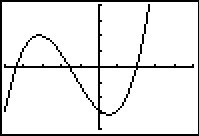
\includegraphics[height=2in]{figures/PolyDiv01.jpg}
    
    &
    
    \setlength\arraycolsep{0.1pt}
    \setlength\extrarowheight{2pt}
    
    $\begin{array}{cccccccccc}
        & & & & & x^2 & + & 6x & + & 7 \\ \hhline{~~~|-------}
        x & - & 2  \vline& x^3 & + & 4x^2 & - & 5x & - & 14 \\
        &  &  -& \left(x^3 \right. & - & \left.  2x^2\right) &  &  &  &  \\ \hhline{~~~---~~~~} 
        &  &  &   &  & 6 x^2 & - & 5x &  &  \\ 
        &  &  &   & - & \left(6 x^2 \right. & - & \left. 12x \right) &  &  \\ \hhline{~~~~~---~~} 
        &  &  &   &   &  & & 7x  & - & 14 \\
        &  &  &   &   &  & - & \left( 7x \right. & - & \left. 14 \right) \\ \hhline{~~~~~~~---} 
        &   &  &  &  &  &  &  &  & 0
    \end{array}$
    
    \setlength\arraycolsep{5pt}
    \setlength\extrarowheight{0pt}  \\

\end{tabular}

Said differently, $f(x) = x^3 + 4x^2-5x-14=(x-2)\left(x^2+6x+7\right)$.  Using this form of $f(x)$, we find the zeros by solving $(x-2)\left(x^2+6x+7\right)=0$.  Setting each factor equal to $0$, we get  $x-2=0$ (which gives us our known zero, $x=2$) as well as $x^2+6x+7=0$.   The latter doesn't factor nicely, so we apply the Quadratic Formula to get $x = -3 \pm \sqrt{2}$.  Sure enough, $-3 - \sqrt{2} \approx -4.414$ and $-3 +\sqrt{2} \approx -1.586$.  We leave it to the reader to show $f(-3-\sqrt{2}) = 0$ and $f(-3+\sqrt{2}) = 0$. % (See Exercise \ref{verifyrootsex}.) 

The point of this section is to generalize the technique applied here.  First up is a friendly reminder of what we can expect when we divide polynomials. 

\begin{theorem}
    \label{polydivthm}
    Suppose $d(x)$ and $p(x)$ are nonzero polynomial functions where the degree of $p$ is greater than or equal to the degree of $d$.  There exist two unique polynomial functions, $q(x)$ and $r(x)$, such that $p(x) = d(x)  q(x) + r(x),$ where either $r(x) = 0$ or the degree of $r$ is strictly less than the degree of $d$. 
\end{theorem}

As you may recall, all of the polynomials in Theorem \ref{polydivthm} have special names.  The polynomial $p$ is called the \index{polynomial division ! dividend} \emph{dividend}; $d$ is the \index{polynomial division ! divisor} \emph{divisor}; $q$ is the \index{polynomial division ! quotient} \emph{quotient}; $r$ is the \index{polynomial division ! remainder} \emph{remainder}.  If $r(x)=0$ then $d$ is called a \index{polynomial division ! factor} \emph{factor} of $p$.  The word `unique' here is critical in that it guarantees there is only \textit{one} quotient and remainder for each division problem.%
\footnote{Hence the use of the definite article `the' when speaking of \textit{the} quotient and \textit{the} remainder.}
The proof of Theorem \ref{polydivthm} is usually relegated to a course in Abstract Algebra, but we can still use the result to move forward with the rest of this section.

If we want to find all of the roots of a polynomial in a reasonable way, we had better find a more efficient way to divide polynomial functions by quantities of the form $x-c$.  Fortunately, people like \href{http://en.wikipedia.org/wiki/Synthetic_division}{Ruffini} and \href{http://en.wikipedia.org/wiki/Horner_scheme}{Horner} have already blazed this trail.  Let's take a closer look at the long division we performed at the beginning of the section and try to streamline it.  First off, let's change all of the subtractions into additions by distributing through the $-1$s.


\setlength\arraycolsep{0.1pt}
\setlength\extrarowheight{2pt}

\[ 
\begin{array}{cccccccccc}
    & & & & & x^2 & + & 6x & + & 7 \\ \hhline{~~~|-------}
    x & - & 2  \vline& x^3 & + & 4x^2 & - & 5x & - & 14 \\
    &  &  &  -x^3  & + &   2x^2 &  &  &  &  \\ \hhline{~~~---~~~~} 
    &  &  &   &  & 6 x^2 & - & 5x &  &  \\ 
    &  &  &   & &-6 x^2  & + &  12x &  &  \\ \hhline{~~~~~---~~} 
    &  &  &   &   &  & & 7x  & - & 14 \\
    &  &  &   &   &  & & - 7x  & + &  14  \\ \hhline{~~~~~~~---} 
    &   &  &  &  &  &  &  &  & 0
\end{array}
\]

\setlength\arraycolsep{5pt}
\setlength\extrarowheight{0pt}


Next, observe that the terms $-x^3$, $-6x^2$ and $-7x$ are the exact opposite of the terms above them.  The algorithm we use ensures this is always the case, so we can omit them without losing any information. Also note that the terms we `bring down' (namely the $-5x$ and $-14$) aren't really necessary to recopy, so we omit them, too.

\setlength\arraycolsep{0.1pt}
\setlength\extrarowheight{2pt}

\[ 
\begin{array}{cccccccccc}
    & & & & & x^2 & + & 6x & + & 7 \\ \hhline{~~~|-------}
    x & - & 2  \vline&   x^3 & + & 4x^2 & - & 5x & - & 14 \\
    &  &  &   &  &   2x^2 &  &  &  &  \\ \hhline{~~~---~~~~} 
    &  &  &   &  & 6 x^2 &  &  &  &  \\ 
    &  &  &   & &  &  &  12x &  &  \\ \hhline{~~~~~---~~} 
    &  &  &   &   &  & & 7x  &  &  \\
    &  &  &   &   &  & &   &  &  14  \\ \hhline{~~~~~~~---} 
    &   &  &  &  &  &  &  &  & 0
\end{array}
\]

\setlength\arraycolsep{5pt}
\setlength\extrarowheight{0pt}

Let's move terms up a bit and copy the $x^3$ into the last row.

\setlength\arraycolsep{0.1pt}
\setlength\extrarowheight{2pt}

\[ 
\begin{array}{cccccccccc}
    
    & & & & & x^2 & + & 6x & + & 7 \\ \hhline{~~~|-------}
    
    x & - & 2  \vline&   x^3 & + & 4x^2 & - & 5x & - & 14 \\
    
    &  &  &   & &   2x^2 &  & 12x &  & 14 \\ \hhline{~~~-------} 
    &  &  & x^3  &  & 6 x^2 &  & 7x &  &0  \\  
\end{array}
\]

\setlength\arraycolsep{5pt}
\setlength\extrarowheight{0pt}

Note that by arranging things in this manner, each term in the last row is obtained by adding the two terms above it.  Notice also that the quotient polynomial can be obtained by dividing each of the first three terms in the last row by $x$ and adding the results.   If you take the time to work back through the original division problem, you will find that this is exactly the way we determined the quotient polynomial.  This means that we no longer need to write the quotient polynomial down, nor the $x$ in the divisor, to determine our answer.

\setlength\arraycolsep{0.1pt}
\setlength\extrarowheight{2pt}

\[ 
\begin{array}{cccccccccc}
    & & - 2   \vline&   x^3 & + & 4x^2 & - & 5x & - & 14 \\
    &  &  &   & &   2x^2 &  & 12x &  & 14 \\ \hhline{~~~-------} 
    &  &  & x^3  &  & 6 x^2 &  & 7x &  &0  \\  
\end{array}
\]

\setlength\arraycolsep{5pt}
\setlength\extrarowheight{0pt}

We've streamlined things quite a bit so far, but we can still do more.  Let's take a moment to remind ourselves where the $2x^2$, $12x$ and $14$ came from in the second row.  Each of these terms was obtained by multiplying the terms in the quotient, $x^2$, $6x$ and $7$, respectively, by the $-2$ in $x-2$,  then by $-1$ when we changed the subtraction to addition.  Multiplying by $-2$ then by $-1$ is the same as multiplying by $2$, so we replace the $-2$ in the divisor by $2$.   Furthermore, the coefficients of the quotient polynomial match the coefficients of the first three terms in the last row, so we now take the plunge and write only the coefficients of the terms to get

\[ 
\begin{array}{rrrrr}
    2   \vline& 1 & 4 & -5  & -14 \\
    &&   2 &   12 &   14 \\ \hhline{~----} 
    & 1  &   6  &  7 &  0  \\  
\end{array}
\]

We have constructed a \index{polynomial division ! synthetic division}\index{synthetic division tableau}\emph{synthetic division tableau} for this polynomial division problem.  Let's re-work our division problem using this tableau to see how it greatly streamlines the division process.  To divide $x^3+4x^2-5x-14$ by $x-2$, we write $2$ in the place of the divisor and the coefficients of $x^3+4x^2-5x-14$ in for the dividend.  Then `bring down' the first coefficient of the dividend.

\begin{center}
    \begin{tabular}{cc}
        $ \begin{array}{rrrrr}
            2   \vline& 1 & 4 & -5  & -14 \\
            &  &    &    &  \\ \hhline{~----} 
            &   &     &   &    \\  
        \end{array}$  \hspace{1in}
        &
        $ \begin{array}{rrrrr}
            2   \vline& 1 & 4 & -5  & -14 \\
            & \downarrow &    &    &  \\ \hhline{~----} 
            & 1  &     &   &    \\  
        \end{array}$ \\
    \end{tabular}
\end{center}

Next, take the $2$ from the divisor and multiply by the $1$ that was `brought down' to get $2$.  Write this underneath the $4$, then add to get $6$.

\begin{center}
    \begin{tabular}{cc}
        $ \begin{array}{rrrrr}
            2   \vline& 1 & 4 & -5  & -14 \\
            & \downarrow  &  2  &    &  \\ \hhline{~----} 
            & 1  &     &   &    \\  
        \end{array}$ \hspace{1in}
        &
        $ \begin{array}{rrrrr}
            2   \vline& 1 & 4 & -5  & -14 \\
            & \downarrow &  2  &    &  \\ \hhline{~----} 
            & 1  &   6  &   &    \\  
        \end{array}$ \\
    \end{tabular}
\end{center}

Now take the $2$ from the divisor times the $6$ to get $12$, and add it to the $-5$ to get $7$.

\begin{center}
    \begin{tabular}{cc}
        $ \begin{array}{rrrrr}
            2   \vline& 1 & 4 & -5  & -14 \\
            & \downarrow &  2  &  12  &  \\ \hhline{~----} 
            & 1  &   6  &   &    \\  
        \end{array}$ \hspace{1in}
        &
        $ \begin{array}{rrrrr}
            2   \vline& 1 & 4 & -5  & -14 \\
            & \downarrow &  2  &  12  &  \\ \hhline{~----} 
            & 1  &   6  & 7  &    \\  
        \end{array}$ \\
    \end{tabular}
\end{center}


Finally, take the $2$ in the divisor times the $7$ to get $14$, and add it to the $-14$ to get $0$.

\begin{center}
    \begin{tabular}{cc}
        $ \begin{array}{rrrrr}
            2   \vline& 1 & 4 & -5  & -14 \\
            & \downarrow &  2  &  12  & 14 \\ \hhline{~----} 
            & 1  &   6  & 7  &    \\  
        \end{array}$ \hspace{1in} 
        &
        $ \begin{array}{rrrrr}
            2   \vline& 1 & 4 & -5  & -14 \\
            & \downarrow &  2  &  12  & 14 \\ \hhline{~----} 
            & 1  &   6  & 7  &  \fbox{$0$}  \\  
        \end{array}$ \\
    \end{tabular}
\end{center}

The first three numbers in the last row of our tableau are the coefficients of the quotient polynomial.  Remember, we started with a third degree polynomial and divided by a first degree polynomial, so the quotient is a second degree polynomial.  Hence the quotient is $x^2+6x+7$.  The number in the box is the remainder.  Synthetic division is our tool of choice for dividing polynomials by divisors of the form $x-c$.  It is important to note that it works \emph{only} for these kinds of divisors.%
\footnote{You'll need to use good old-fashioned polynomial long division for divisors of degree larger than 1.} 
Also take note that when a polynomial (of degree at least $1$) is divided by $x-c$, the result will be a polynomial of exactly one less degree. Finally, it is  worth the time to trace each step in synthetic division back to its corresponding step in long division.  While the authors have done their best to indicate where the algorithm comes from, there is no substitute for working through it yourself.

\begin{example}  
    Use synthetic division to perform the following polynomial divisions.  Identify the quotient and remainder. 
    \begin{multicols}{3}
        \begin{enumerate}
            \item  $\left(5x^3 - 2x^2 + 1\right) \div (x-3)$ \vphantom{$\dfrac{4-8x-12x^2}{2x-3}$}
            \item  $\left(t^3+8\right) \div (t+2)$ \vphantom{$\dfrac{4-8x-12x^2}{2x-3}$}
            \item  $\dfrac{4-8z-12z^2}{2z-3}$
        \end{enumerate}
    \end{multicols}
\end{example}

\begin{exampleSol}
    \begin{enumerate}
        \item When setting up the synthetic division tableau, the coefficients of even `missing' terms need to be accounted for, so we enter $0$ for the coefficient of $x$ in the dividend.  
            \[ 
            \begin{array}{rrrrr}
                3   \vline& 5 & -2 & 0  & 1 \\
                & \downarrow &  15  &  39  & 117 \\ \hhline{~----} 
                & 5  &   13  & 39  &  \fbox{$118$}  \\  
            \end{array}
            \]
            Since the dividend was a third degree polynomial function, the quotient is a second degree (quadratic) polynomial function with coefficients $5$, $13$ and $39$:   $q(x) = 5x^2+13x+39$. The remainder is $r(x) = 118$.  According to Theorem \ref{polydivthm}, we have $5x^3 - 2x^2 + 1 = (x-3)\left(5x^2+13x+39 \right) + 118$, which we leave to the reader to check.
        
        \item  To use synthetic division here, we rewrite $t+2$ as $t-(-2)$ and proceed as before
            \[ 
                \begin{array}{rrrrr}
                    -2   \vline& 1 & 0 & 0  & 8 \\
                    & \downarrow &  -2  &  4  & -8 \\ \hhline{~----} 
                    & 1  &   -2  & 4  &  \fbox{$0$}  \\  
                \end{array}
            \]
            We get the quotient $q(t) = t^2-2t+4$ and the remainder $r(t) =0$. Relating the dividend, quotient and remainder gives: $t^3+8 = (t+2)\left( t^2-2t+4 \right)$, which is a specific instance of the `sum of cubes' formula some of you may recall.  
        
        \item To divide $4-8z-12z^2$ by $2z-3$, two things must be done.  First, we write the dividend in descending powers of $z$ as $-12z^2-8z+4$.  Second, since synthetic division works only for factors of the form $z-c$, we factor $2z-3$ as $2\left(z-\frac{3}{2}\right)$.  Hence, we are dividing  $-12z^2-8z+4$ by two factors:  $2$ and $\left(z-\frac{3}{2}\right)$.  Dividing first by $2$, we obtain $-6z^2-4z+2$.  Next, we divide  $-6z^2-4z+2$ by $\left(z-\frac{3}{2}\right)$:
            \[ 
                \begin{array}{rrrr}
                    \frac{3}{2}   \vline& -6 & -4 & 2   \\ [4pt]
                    & \downarrow &  -9  & -\frac{39}{2}  \\ [4pt] \hhline{~---} 
                    &  -6  &   -13  & \fbox{$-\frac{35}{2}$}  \\  
                \end{array}
            \]
            Hence,  $-6z^2-4z+2 = \left(z-\frac{3}{2}\right)(-6 z - 13) - \frac{35}{2}$.  However when it comes to writing  the dividend, quotient and remainder in the form given in Theorem \ref{polydivthm}, we need to find $q(z)$ and $r(z)$ so that  $-12z^2-8z+4 = (2z-3) q(z) + r(z)$. Hence, starting with $-6z^2-4z+2 = \left(z-\frac{3}{2}\right)(-6 z - 13) - \frac{35}{2}$, we multiply $2$ back on both sides:  
            \[ 
                \begin{array}{rcl}
                    -6z^2-4z+2  & = & \left(z-\frac{3}{2}\right)(-6 z - 13) - \frac{35}{2}\\
                    2\left(-6z^2-4z+2 \right) & = & 2 \left[ \left(z-\frac{3}{2}\right)(-6 z - 13) - \frac{35}{2} \right] \\
                    -12z^2-8z+4 & = & 2 \left(z-\frac{3}{2}\right)(-6 z - 13) - 2 \left(\frac{35}{2} \right) \\
                    -12z^2-8z+4 & = & (2z-3) (-6 z - 13) - 35  \\ 
                \end{array} 
            \]
            At this stage, we have written $-12z^2-8z+4$ in the \emph{form} $(2z-3) q(z) + r(z)$, so we identify the quotient as  $q(z) = -6z-13$ and the remainder is $r(z) = -35$.  But how can we be sure these are the same quotient and remainder polynomial functions we would have obtained if we had taken the time to do the long division in the first place?   Because of the word   `unique' in Theorem \ref{polydivthm}.  The theorem states that there is only \textit{one} way to decompose $-12z^2-8z+4$ as $(2z-3)q(z) + r(z)$.  Since we have found such a way, we can be sure it is the only way.\footnote{But it wouldn't hurt to check, just this once.}
    \end{enumerate}
\end{exampleSol}

The next example pulls together all of the concepts discussed in this section.  

\begin{example} 
    Let $p(x) = 2x^3-5x+3$.
    \begin{enumerate}
        \item  Find $p(-2)$ using The Remainder Theorem.  Check your answer by substitution.
        \item  Verify  $x=1$ is a zero of $p$ and use this information to all the real zeros of $p$.
    \end{enumerate}
\end{example}

\begin{exampleSol}
    \begin{enumerate}
        \item  The Remainder Theorem states $p(-2)$ is the remainder when $p(x)$ is divided by $x-(-2)$.  We set up our synthetic division tableau below.  We are careful to record the coefficient of $x^2$ as $0$:
        \[
            \begin{array}{rrrrr}
                -2   \vline& 2 & 0 & -5  & 3 \\
                & \downarrow &  -4  &  8  & -6 \\ \hhline{~----} 
                & 2  &   -4  & 3 &  \fbox{$-3$}  \\  
            \end{array}
        \]
        According to the Remainder Theorem, $p(-2) = -3$.  We can check this by direct substitution into the formula for $p(x)$:  $p(-2) = 2(-2)^3-5(-2)+3 = -16+10+3=-3$.
        
        \item We verify $x=1$ is a zero of $p$ by evaluating $p(1) = 2(1)^3-5(1)+3 = 0$.  To see if there are any more real zeros, we need to solve $p(x) = 2x^3-5x+3 = 0$.  From the Factor Theorem, we know since $p(1) = 0$,  we can factor $p(x)$ as $(x-1)q(x)$.  To find $q(x)$, we use synthetic division:
            
            \[
                \begin{array}{rrrrr}
                    1   \vline& 2 & 0 & -5  & 3 \\
                    & \downarrow &  2  &  2  & -3 \\ \hhline{~----} 
                    & 2  &   2  & -3 &  \fbox{$0$}  \\  
                \end{array}
            \]
            As promised, our remainder is $0$, and we get  $p(x) = (x-1)\left( 2x^2 + 2x - 3\right)$.  Setting this form of $p(x)$ equal to  $0$ we get $(x-1)\left( 2x^2 + 2x - 3\right) = 0$.  We recover  $x = 1$ from setting $x-1=0$  but we also obtain $x = \frac{-1 \pm \sqrt{7}}{2}$ from  $2x^2 + 2x - 3=0$, courtesy of the Quadratic Formula.  
    \end{enumerate}
\end{exampleSol}

Our next example demonstrates how we can extend the synthetic division tableau to accommodate zeros of multiplicity greater than $1$.

\begin{example}  
    Let $p(x) = 4x^4-4x^3-11x^2+12x-3$. Show $x=\frac{1}{2}$ is a zero of multiplicity $2$ and find all of the remaining real zeros of $p$.
\end{example}

\begin{exampleSol}
    While computing $p\left(\frac{1}{2} \right) = 0$ shows $x=\frac{1}{2}$  is a zero of $p$, to prove it has multiplicity $2$, we need to factor $p(x) = \left(x - \frac{1}{2}\right)^2 q(x)$ with $q\left( \frac{1}{2} \right) \neq 0$,.   We set up for synthetic division, but instead of stopping after the first division, we continue the tableau downwards and divide $\left(x - \frac{1}{2}\right)$ directly into the quotient we obtained from the first division as follows:
    \[
        \begin{array}{rrrrrr}
            \frac{1}{2}   \vline& 4 & -4 & -11  & 12 & -3 \\
            & \downarrow &  2  &  -1  & -6 & 3\\ \hhline{~-----} \frac{1}{2}   \vline&  4  &   -2  & -12 & 6 &  \fbox{$0$}  \\
            & \downarrow &  2  &  0  & -6 &\\ \hhline{~----} & 4  &   0  & -12 & \fbox{0} &   \\  
        \end{array}
    \]
    
    \setlength\arraycolsep{5pt}
    \setlength\extrarowheight{0pt}
    
    We get:%
    \footnote{
        For those wanting more detail:  the first division gives:  $4x^4-4x^3-11x^2+12x-3=\left(x-\frac{1}{2}\right) \left(4x^3-2x^2-12x+6\right)$.  The second division gives: $4x^3-2x^2-12x+6=\left(x-\frac{1}{2}\right)\left(4x^2-12\right)$.
        }
    $4x^4-4x^3-11x^2+12x-3 = \left(x-\frac{1}{2}\right)^2\left(4x^2-12\right)$.  Note if we let $q(x) = 4x^2-12$, then $q\left(\frac{1}{2} \right) = 4\left(\frac{1}{2} \right)^2 - 12 = -11 \neq 0$  which proves $x = \frac{1}{2}$ is a zero of $p$ of multiplicity $2$.   To find the remaining zeros of $p$, we set the quotient $4x^2-12=0$, so $x^2 = 3$ and extract square roots to get $x = \pm \sqrt{3}$. 
\end{exampleSol} 

One last wrinkle in this process is complex roots, since it is possible for a polynomial (particularly a quadratic polynomial) to have complex numbers as roots. For a reminder of some more properties of complex numbers see \sectionref{sec:complexNums}. For this section in particular, we only need a few basic facts.

For us, it suffices to review the basic vocabulary.

\begin{definition}  
    \begin{itemize}
         \item The imaginary unit $i = \sqrt{-1}$ satisfies the two following properties
        \begin{enumerate}
            \item  $i^2 = -1$
            \item  If $c$ is a real number with $c \geq 0$ then $\sqrt{-c} = i \sqrt{c}$
        \end{enumerate}
        \item The \emph{complex numbers} are the set of numbers $\mathbb{C} = \{ a + bi  |  a, b \in \mathbb{R} \}$
        \item  Given a complex number $z = a+bi$, the \emph{complex conjugate} of $z$, $\overline{z}  = \overline{a+bi} = a - bi$.
    \end{itemize}
\end{definition}

Note that every real number is a complex number, that is $\mathbb{R} \subseteq \mathbb{C}$.  To see this, take your favorite real number, say $117$.  We may write $117 = 117 + 0 i$ which puts in the form $a + bi$.  Hence, we we speak of the `complex zeros' of a polynomial function, we are talking about not just the non-real, but also the real zeros.

Complex numbers, by their very definition, are two dimensional creatures.  To see this, we may identify a complex number $z = a+bi$ with the point in the Cartesian plane $(a,b)$. The horizontal axis is called the `real' axis since points here have the form $(a,0)$ which corresponds to numbers of the form $z = a + 0i = a$ which are the real numbers. The vertical axis is called the `imaginary' axis since points here are of the form $(0,b)$ which correspond to numbers of the form $z = 0+bi = bi$,  the so-called `purely imaginary' numbers.  Below we plot some complex numbers on this so-called  `Complex Plane.'  Plotting a set of complex numbers this way is called an \href{https://en.wikipedia.org/wiki/Complex_plane}{Argand Diagram}, and opens up a wealth of opportunities to explore many algebraic properties of complex numbers geometrically. For example, complex conjugation amounts to a reflection about the real axis, and multiplication by $i$ amounts to a $90^{\circ}$ rotation. While we won't have much use for the Complex Plane in this section, it is worth introducing this concept now, if, for no other reason, it gives the reader a sense of the vastness of the complex number system and the role of the real numbers in it.

% \begin{center}
%\begin{mfpic}[15]{-5}{5}{-5}{5}
%\axes
%\tlabel[cl](5,-0.5){\scriptsize Real Axis}
%\tlabel[cl](0.5,5){\scriptsize Imaginary Axis}
%\xmarks{-4,-3,-2,-1,1,2,3,4}
%\ymarks{-4,-3,-2,-1,1,2,3,4}
%\point[3pt]{(0,0),(3,0), (-4,2), (0,-3)}
%\tlabel[cc](-4,2.5){\scriptsize $(-4,2) \longleftrightarrow z = -4+2i$}
%\tlabel[cl](0.25,-3){\scriptsize $(0,-3) \longleftrightarrow z = -3i$}
%\tlabel[cc](3,0.5){\scriptsize $(3,0) \longleftrightarrow z = 3$}
%\tlabel[cc](0.25,-0.35){\scriptsize $0$}
%\tlpointsep{5pt}
%\scriptsize
%\tcaption{\scriptsize The Complex Plane}
% \axislabels {x}{{$-4 \hspace{7pt}$} -4, {$-3 \hspace{7pt} $} -3, {$-2\hspace{7pt} $} -2, {$-1 \hspace{7pt}$} -1, {$1$} 1, {$2$} 2, {$3$} 3, {$4$} 4}
% \axislabels {y}{{$-4i$} -4, {$-3i$} -3, {$-2i$} -2, {$-i$} -1, {$i$} 1, {$2i$} 2, {$3i$} 3, {$4i$} 4}
% \normalsize
% \end{mfpic}
% \end{center}

Returning to zeros of polynomials, suppose we wish to find the zeros of $f(x) = x^2-2x+5$.  To solve the equation $x^2-2x+5 = 0$, we note that the quadratic doesn't factor nicely, so we resort to the Quadratic Formula %, Equation \ref{quadraticformulafunction}
and obtain 
\[ 
    x = \dfrac{-(-2) \pm \sqrt{(-2)^2-4(1)(5)}}{2(1)} = \dfrac{2 \pm \sqrt{-16}}{2} = \dfrac{2 \pm 4i}{2} = 1 \pm 2i.
\] 
Two things are important to note.  First, the zeros $1+2i$ and $1-2i$ are complex conjugates.  If ever we obtain non-real zeros to a quadratic function with \textit{real number} coefficients, the zeros  will be a complex conjugate pair. (Do you see why?)  

We could ask if all of the theory of polynomial division % from Section\ref{Polydivision} 
holds for non-real zeros, in particular the division algorithm and the Remainder and Factor Theorems.  The answer is `yes.'  

\[
    \begin{array}{rrrr}
        1+2i   \vline & 1 & -2 & 5 \\
        & \downarrow   &  1+2i  &  -5 \\ \hhline{~---} 
        & 1 & -1+2i &  \fbox{$0$}   \\
    \end{array}
\]

Indeed, the above shows $x^2-2x+5  = (x-[1+2i])(x-1+2i)= (x-[1+2i])(x-[1-2i])$ which demonstrates both  $(x-[1+2i])$ and  $(x-[1-2i])$ are factors of $x^2-2x+5$.%
\footnote{
    It is a good review of the algebra of complex numbers to start with  $(x-[1+2i])(x-[1-2i])$, perform the indicated operations, and simplify the result to $x^2-2x+5$.  See part 6 of  Example \ref{complexzeroex1}.
    }%  in Section  \ref{AppCmpNums}.}

But how do we know if a general polynomial has any complex zeros at all?  We have many examples of polynomials with no real zeros.  Can there be polynomials with no zeros whatsoever?  The answer to that last question is ``No.'' and the theorem which provides that answer is \index{Fundamental Theorem of Algebra} The Fundamental Theorem of Algebra.

\begin{theorem}[The Fundamental Theorem of Algebra]
    \label{ftoa}
    Suppose $f$ is a polynomial function with complex number coefficients of degree $n \geq 1$, then $f$ has at least one complex zero.
\end{theorem}

The Fundamental Theorem of Algebra is an example of an `existence' theorem in Mathematics.  Like the Intermediate Value Theorem, % Theorem \ref{IVT},
the Fundamental Theorem of Algebra  guarantees the existence of at least one zero, but gives us no algorithm to use in finding it.  In fact, as we mentioned previously, there are polynomials whose real zeros, though they exist, cannot be expressed using the `usual' combinations of arithmetic symbols, and must be approximated.  It took mathematicians literally hundreds of years to prove the theorem in its full generality,%
\footnote{So if its profound nature and beautiful subtlety escape you, no worries!} 
and some of that history is recorded \href{http://en.wikipedia.org/wiki/Fundamental_theorem_of_algebra}{\underline{here}}.  Note that the Fundamental Theorem of Algebra  applies to not only polynomial functions with real coefficients, but to those with complex number coefficients as well.  

Suppose  $f$ is a polynomial function of degree $n \geq 1$.  The Fundamental Theorem of Algebra guarantees us at least one complex zero, $z_{\mbox{\tiny $1$}}$.  The Factor Theorem guarantees that $f(x)$ factors as $f(x) = \left(x - z_{\mbox{\tiny $1$}}\right) q_{\mbox{\tiny $1$}}(x)$ for a polynomial function $q_{\mbox{\tiny $1$}}$,  which has degree $n-1$.  If $n-1 \geq 1$, then the Fundamental Theorem of Algebra guarantees a complex zero of $q_{\mbox{\tiny $1$}}$ as well, say $z_{\mbox{\tiny $2$}}$, so then the Factor Theorem gives us $q_{\mbox{\tiny $1$}}(x) = \left(x - z_{\mbox{\tiny $2$}}\right) q_{\mbox{\tiny $2$}}(x)$, and hence $f(x) = \left(x - z_{\mbox{\tiny $1$}}\right) \left(x - z_{\mbox{\tiny $2$}}\right) q_{\mbox{\tiny $2$}}(x)$.  We can continue this process exactly $n$ times, at which point our quotient polynomial $q_{\mbox{\tiny $n$}}$ has degree $0$ so it's a constant.  This constant is none-other than the leading coefficient of $f$ which is carried down line by line each time we divide by factors of the form $x-c$.


\begin{theorem}[Complex Factorization Theorem] 
    \label{complexfactorization}
    Suppose $f$ is a polynomial function with complex number coefficients.  If the degree of $f$ is $n$ and $n \geq 1$, then  $f$ has exactly $n$ complex zeros, counting multiplicity.  If 
    $z_{\mbox{\tiny $1$}}$, $z_{\mbox{\tiny $2$}}$, \ldots, $z_{\mbox{\tiny $k$}}$ 
    are the distinct zeros of $f$, with multiplicities $m_{\mbox{\tiny $1$}}$, $m_{\mbox{\tiny $2$}}$, \ldots, $m_{\mbox{\tiny $k$}}$, respectively, then 
    $f(x) = a\left(x - z_{\mbox{\tiny $1$}}  \right)^{m_{\mbox{\tiny $1$}}}\left(x - z_{\mbox{\tiny $2$}}  \right)^{m_{\mbox{\tiny $2$}}} \cdots \left(x - z_{\mbox{\tiny $k$}}  \right)^{m_{\mbox{\tiny $k$}}}$. 
    \index{Complex Factorization Theorem}
\end{theorem}


Theorem \ref{complexfactorization} says two important things:  first, every polynomial is a product of linear factors;  second, every polynomial function is completely determined by its zeros, their multiplicities, and its leading coefficient.  We put this theorem to good use in the next example.

\begin{example}  
    Let $f(x) = 12x^5 - 20x^4+19x^3-6x^2-2x+1$.
    \begin{enumerate}
        \item Find all of the complex zeros of $f$ and state their multiplicities.  
        \item  Factor $f(x)$ using Theorem \ref{complexfactorization}
    \end{enumerate}
\end{example}

\begin{exampleSol}
\begin{enumerate}
\item  Since $f$ is a fifth degree polynomial, we know that we need to perform at least three successful divisions to get the quotient down to a quadratic function.  At that point, we can find the remaining zeros using the Quadratic Formula, if necessary.  Using the techniques of synthetic division: % developed in Section \ref{RealZeros}:
\[
\begin{array}{rrrrrrr}
    \frac{1}{2}   \vline& 12 & -20& 19  & -6 & -2 &1 \\
    & \downarrow     &  6  &  -7  & 6 & 0 & -1\\ \hhline{~------} \frac{1}{2}   \vline& 12 & -14 & 12  & 0 & -2 & \fbox{$0$} \\
    & \downarrow     &  6 &  -4  & 4 & 2 &\\ \hhline{~-----} -\frac{1}{3}   \vline&  12 &  -8  & 8 & 4 &  \fbox{$0$} & \\
    & \downarrow &  -4  &  4  & -4  & & \\ \hhline{~----} & 12  &   -12 & 12& \fbox{0} &&   \\
\end{array}
\]

Our quotient is $12x^2 - 12x + 12$, whose zeros we find to be $\frac{1 \pm i \sqrt{3}}{2}$.  From Theorem \ref{complexfactorization}, we know $f$ has exactly $5$ zeros, counting multiplicities, and as such we have the zero $\frac{1}{2}$ with multiplicity $2$, and the zeros $-\frac{1}{3}$, $\frac{1 + i \sqrt{3}}{2}$ and $\frac{1 - i \sqrt{3}}{2}$, each of multiplicity $1$.

\item  Applying Theorem \ref{complexfactorization}, we are guaranteed that $f$ factors as
\[
    f(x) = 12 \left(x- \dfrac{1}{2}\right)^2 \left(x + \dfrac{1}{3}\right) \left(x - \left[\dfrac{1 + i \sqrt{3}}{2}\right]\right) \left(x - \left[\dfrac{1 - i \sqrt{3}}{2}\right]\right)
\]
\end{enumerate}

\end{exampleSol}

A true test of Theorem \ref{complexfactorization} would be to take the factored form of $f(x)$ in the previous example and multiply it out%
\footnote{This is a good chance to test your algebraic mettle and see that all of this does actually work.} 
to see that it really does reduce to  $f(x) = 12x^5 - 20x^4+19x^3-6x^2-2x+1$.  When factoring a polynomial using Theorem \ref{complexfactorization}, we say that it is \index{polynomial function ! completely factored ! over the complex numbers} \emph{factored completely over the complex numbers}, meaning that it is impossible to factor the polynomial any further using complex numbers.  If we wanted to  \index{polynomial function ! completely factored ! over the real numbers} completely factor $f(x)$ over the \emph{real numbers} then we would have stopped short of finding the nonreal zeros of $f$ and factored $f$ using our work from the synthetic division to write $f(x) = \left(x - \frac{1}{2} \right)^2 \left(x + \frac{1}{3} \right)\left(12x^2 - 12x + 12\right)$, or $f(x) = 12\left(x - \frac{1}{2} \right)^2 \left(x + \frac{1}{3} \right)\left(x^2 - x + 1\right)$.  Since the zeros of $x^2-x+1$ are nonreal, we call $x^2-x+1$ an \index{quadratic function ! irreducible quadratic}\index{irreducible quadratic}\emph{irreducible quadratic} meaning it is impossible to break it down any further using \emph{real} numbers.  


The last two results of the section show us that, theoretically, the non-real zeros of polynomial functions with real number coefficients come exclusively from irreducible quadratics.

\begin{theorem}[Conjugate Pairs Theorem] 
    \label{conjugatepairsthm}
    If $f$ is a polynomial function with real number coefficients and $z$ is a complex zero of $f$, then so is $\overline{z}$. \index{Conjugate Pairs Theorem}
\end{theorem}


To prove the theorem, let $ f(x) = a_{n} x^{n} + a_{n-\mbox{\tiny$1$}} x^{n-\mbox{\tiny$1$}} + \ldots + a_{\mbox{\tiny $2$}} x^{\mbox{\tiny $2$}} + a_{\mbox{\tiny $1$}} x + a_{\mbox{\tiny $0$}}$ be a polynomial function with real number coefficients.  If $z$ is a zero of $f$, then $f(z) = 0$, which means $a_{n} z^{n} + a_{n-\mbox{\tiny$1$}} z^{n-\mbox{\tiny$1$}} + \ldots + a_{\mbox{\tiny $2$}} z^{\mbox{\tiny $2$}} + a_{\mbox{\tiny $1$}} z + a_{\mbox{\tiny $0$}} = 0$.  Next, we consider $f\left(\overline{z}\right)$ and apply Theorem \ref{conjugateprops} below.

\[ 
\begin{array}{rclr}
    f\left(\overline{z}\right) & = &  a_{n} \left(\overline{z}\right)^{n} + a_{n-\mbox{\tiny$1$}} \left(\overline{z}\right)^{n-\mbox{\tiny$1$}} + \ldots + a_{\mbox{\tiny $2$}}\left( \overline{z}\right)^{\mbox{\tiny $2$}} + a_{\mbox{\tiny $1$}} \overline{z} + a_{\mbox{\tiny $0$}} & \\ [3pt]
    &  = & a_{n}\overline{z^{n}} + a_{n-\mbox{\tiny$1$}}\overline{z^{n-\mbox{\tiny$1$}}} + \ldots + a_{\mbox{\tiny $2$}}\overline{z^{\mbox{\tiny $2$}}} + a_{\mbox{\tiny $1$}} \overline{z} + a_{\mbox{\tiny $0$}} & \mbox{ since $\left(\overline{z}\right)^n = \overline{z^{n}}$}\\ [3pt]
    & = & \overline{a_{n}}\overline{z^{n}} + \overline{a_{n-\mbox{\tiny$1$}}}\overline{z^{n-\mbox{\tiny$1$}}} + \ldots +  \overline{a_{\mbox{\tiny $2$}}}\overline{z^{\mbox{\tiny $2$}}} + \overline{a_{\mbox{\tiny $1$}}} \overline{z} + \overline{a_{\mbox{\tiny $0$}}} & \mbox{since the coefficients are real} \\ [3pt]
    & = & \overline{a_{n} z^{n}} + \overline{a_{n-\mbox{\tiny$1$}} z^{n-\mbox{\tiny$1$}}} + \ldots +  \overline{a_{\mbox{\tiny $2$}} z^{\mbox{\tiny $2$}}} + \overline{a_{\mbox{\tiny $1$}} z} + \overline{a_{\mbox{\tiny $0$}}} &  \mbox{ since $\overline{z}  \overline{w}=\overline{zw} $}\\ [3pt]
    & = & \overline{a_{n} z^{n} + a_{n-\mbox{\tiny$1$}} z^{n-\mbox{\tiny$1$}} + \ldots + a_{\mbox{\tiny $2$}} z^{\mbox{\tiny $2$}} + a_{\mbox{\tiny $1$}} z + a_{\mbox{\tiny $0$}}} & \mbox{ since $ \overline{z} + \overline{w} = \overline{z+w} $}\\ [3pt]
    & = & \overline{f(z)} & \\ [3pt]
    & = & \overline{0} & \\ [3pt]
    & = & 0 & \\
\end{array} 
\]

This shows that $\overline{z}$ is a zero of $f$.  So, if $f$ is a polynomial function with real number coefficients, Theorem \ref{conjugatepairsthm} tells us that if $a+bi$ is a nonreal zero of $f$, then so is $a-bi$.  In other words, nonreal zeros of $f$ come in conjugate pairs.  The Factor Theorem kicks in to give us both $(x-[a+bi])$ and $(x-[a-bi])$ as factors of $f(x)$ which means $(x-[a+bi])(x-[a-bi]) = x^2 + 2a x + \left(a^2+b^2\right)$ is an irreducible quadratic factor of $f$.  As a result, we have our last theorem of the section.

\begin{theorem}[Real Factorization Theorem] 
    \label{realfactorization}
    Suppose $f$ is a polynomial function with real number coefficients.  Then $f(x)$ can be factored into a product of linear factors corresponding to the real zeros of $f$ and irreducible quadratic factors which give the nonreal zeros of $f$. \index{Real Factorization Theorem}
\end{theorem}


\begin{example}  Let $f(x) = x^4+64$.  
\begin{enumerate}
\item  Use synthetic division to show that $x=2+2i$ is a zero of $f$.
\item  Find the remaining complex zeros of $f$.
\item  Completely factor $f(x)$ over the complex numbers.
\item  Completely factor $f(x)$ over the real numbers.
\end{enumerate}
\end{example}

\begin{exampleSol}
    \begin{enumerate}
        \item  Remembering to insert the $0$'s in the synthetic division tableau we have
            \[ 
            \begin{array}{cccccc}
                2+2i   \vline& 1 & 0 & 0  & 0 & 64 \\
                & \downarrow     &  2+2i  &  8i & -16+16i & -64\\ \hhline{~-----} 
                & 1 &  2+2i  & 8i & -16+16i &  \fbox{$0$}  \\ 
            \end{array}
            \]
        
        \item  Since $f$ is a fourth degree polynomial, we need to make two successful divisions to get a quadratic quotient.  Since $2+2i$ is a zero, we know from Theorem \ref{conjugatepairsthm} that $2-2i$ is also a zero.  We continue our synthetic division tableau.
            
            \[ 
            \begin{array}{cccccc}
                2+2i   \vline& 1 & 0 & 0  & 0 & 64 \\
                & \downarrow     &  2+2i  &  8i & -16+16i & -64\\ \hhline{~-----} 
                2-2i   \vline  & 1 &  2+2i  & 8i & -16+16i &  \fbox{$0$}  \\
                & \downarrow &  2-2i  &  8-8i  & 16-16i &\\ \hhline{~----} 
                & 1  &  4  & 8& \fbox{0} &   \\
            \end{array}
            \]
            Our quotient polynomial is $x^2+4x+8$.  Using the quadratic formula, we solve $x^2+4x+8 = 0$ and find the remaining zeros are $-2+2i$ and $-2-2i$.  
        
        \item  Using Theorem \ref{complexfactorization}, we get $f(x) = (x-[2-2i])(x-[2+2i])(x-[-2+2i])(x-[-2-2i])$.
        
        \item  To find the irreducible quadratic factors of $f(x)$, we multiply the factors together which correspond to the conjugate pairs.  We find $(x-[2-2i])(x-[2+2i]) = x^2-4x+8$, and $(x-[-2+2i])(x-[-2-2i]) = x^2+4x+8$, so  $f(x) =  \left(x^2-4x+8\right) \left(x^2+4x+8\right)$.   
    \end{enumerate}
\end{exampleSol}

We close this section with an example where we are asked to manufacture a polynomial function with certain characteristics.

\begin{example}  
    Find a polynomial function $p$ of lowest degree that has integer coefficients and satisfies all of the following criteria:
    \begin{itemize}
        \item  the graph of $y=p(x)$ touches and rebounds from the $x$-axis at $\left(\frac{1}{3}, 0\right)$
        \item  $x=3i$ is a zero of $p$.
        \item  as $x \rightarrow -\infty$, $p(x) \rightarrow -\infty$
        \item  as $x \rightarrow \infty$, $p(x) \rightarrow -\infty$
    \end{itemize}
    % \item  Find a possible formula for the polynomial function $p$ graphed below.  You may leave your answer in factored form.
    %\begin{center}
    %\begin{mfpic}[15]{-5}{5}{-6}{6}
    %\axes
    %\tlabel[cc](5,-0.5){\scriptsize $t$}
    %\tlabel[cc](0.5,6){\scriptsize $y$}
    %\xmarks{-4, -3,-2,-1,1,2,3,4}
    %\ymarks{-5,-4,-3,-2,-1,1,2,3,4,5}
    %\tlpointsep{5pt}
    %\scriptsize
    %\axislabels {x}{{$-4 \hspace{7pt}$} -4, {$-3 \hspace{7pt}$} -3,{$-2 \hspace{7pt}$} -2, {$-1 \hspace{7pt}$} -1, {$1$} 1, {$2$} 2, {$3$} 3, {$4$} 4}
    %\axislabels {y}{{$-5$} -5,{$-4$} -4,{$-3$} -3,{$-2$} -2,{$-1$} -1, {$1$} 1, {$2$} 2, {$3$} 3, {$4$} 4, {$5$} 5}
    %\normalsize
    %\penwd{1.5pt}
    %\arrow \reverse \arrow \function{-3.6, 2.75, 0.1}{(x**3+x**2-5*x+3)/3}
    % \end{mfpic}
    %\end{center}
\end{example}

\begin{exampleSol}
    
    To solve this problem, we will need a good understanding of the relationship between the $x$-intercepts of the graph of a function and the zeros of a function, the Factor Theorem, the role of multiplicity, complex conjugates, the Complex Factorization Theorem, and end behavior of polynomial functions.  (In short, you'll need most of the major concepts of this chapter.)  Since the graph of $p$ touches the $x$-axis at $\left(\frac{1}{3}, 0\right)$, we know $x=\frac{1}{3}$ is a zero of even multiplicity.  Since we are after a polynomial of lowest degree, we need $x=\frac{1}{3}$ to have multiplicity exactly $2$. The Factor Theorem now tells us  $\left(x-\frac{1}{3}\right)^2$ is a factor of $p(x)$.  Since $x=3i$ is a zero and our final answer is to have integer (hence, real) coefficients, $x=-3i$ is also a zero.  The Factor Theorem kicks in again to give us $(x-3i)$ and $(x+3i)$ as factors of $p(x)$.  We are given no further information about zeros or intercepts so we conclude, by the Complex Factorization Theorem that $p(x) = a \left(x-\frac{1}{3}\right)^2 (x-3i)(x+3i)$ for some real number $a$.  Expanding this, we get $p(x) =  ax^4-\frac{2a}{3} x^3+\frac{82a}{9} x^2-6ax+a$.  In order to obtain integer coefficients, we know $a$ must be an integer multiple of $9$.  Our last concern is end behavior.  Since the leading term of $p(x)$ is $ax^4$, we need $a < 0$ to get $p(x) \rightarrow -\infty$ as $x \rightarrow \pm \infty$. Hence, if we choose $x=-9$, we get $p(x) = -9x^4+ 6 x^3 - 82 x^2+54x-9$.    We can verify our handiwork using the techniques developed in this chapter.  
    
    % \item The first thing to note is the independent variable here is $t$, not $x$ as evidenced by the labeling on the horizontal axis.   Next, the graph appears to cross through the $t$-axis at $(-3,0)$ in a fairly linear fashion, so $t=-3$ is likely a zero of multiplicity $1$.   Also, the graph touches and rebounds at $(1,0)$, indicating $t=1$ is a zero of even multiplicity.  Since the graph doesn't appear too `flat,' we'll go with multiplicity $2$ (though there is really no way of telling.)     Using the Complex Factorization Theorem and assuming we have no non-real zeros, we now have $p(t) = a (t-(-3))(t-1)^2 = a(t+3)(t-1)^2$.  To determine the leading coefficient, $a$, we note the graph appears to have a $y$-intercept at $(0,1)$.  Solving $p(0) = 1$ gives $a(3)(-1)^2 = 1$ or $3a = 1$.  Hence, $a = \frac{1}{3}$ so $p(t) = \frac{1}{3} (t+3)(t-1)^2$. Since we may leave our answer in factored form, we are done.   

\end{exampleSol}

\end{document}






